% -*- root: ../../../main.tex -*-
\subsection{Leader Election}
\label{Leader Election}
In un dato term, tutte le \textit{operazioni di replicazione} del log sono affidate ad un server che ricopre il ruolo di \textit{leader}. Al fine di accordarsi in maniera safe su un unico leader è necessario applicare un protocollo di elezione robusto.  

	\subsubsection{Candidatura}
	Ogni elezione ha inizio nel momento in cui uno o più server si candidano come aspiranti leader.

	\begin{enumerate}
		\item{\textbf{Stato iniziale:}}	ogni server inizialmente si trova nello stato di follower e vi resta fintantochè riceve nuovi messaggi dall'attuale server leader.
		\item{\textbf{Heartbeat:}} il leader, periodicamente, invia un messaggio detto di \textit{heartbeat}\footnote{come heartbeat vengono utilizzati i messaggi di tipo AppendEntries che, nel caso in cui non ci sia effettivamente una entry da appendere, vengono lasciati vuoti.} 
		per comunicare ai suoi follower che è ancora in funzione.
		\item{\textbf{Timeout:}} i server \textbf{follower} mantengono internamente un \textbf{timer randomico} che si resetta ogni volta che viene ricevuto un messaggio dal leader. La durata di questo timer viene chiamata \textit{election timeout}.		
		\item{\textbf{Inizio candidatura:}} allo scadere del timer, il follower considera il leader assente e si propone come leader effettuando un \textbf{cambiamento di stato} da follower a candidate e dando inizio a una \textbf{nuova leader election}.
	\end{enumerate}


Quando una \textit{Leader Election} ha inizio il follower esegue i seguenti passaggi:

\begin{enumerate}
	\item{}
\end{enumerate}
 incrementa il proprio term di uno e cambia il suo stato in candidate, dopodiché vota per sé stesso e procede ad inviare delle \textit{Request Vote} a tutti i membri del cluster.
A questo punto possono verificarsi i seguenti tre scenari:
\begin{enumerate}
	\item Il \textbf{Candidate} vince le elezioni e diventa \textbf{Leader}: questo accade quando il numero di voti ricevuti raggiunge la maggioranza, considerando anche il suo voto.
	\item Un altro \textbf{Candidate} vince l'elezione: questo può accadere se ad esempio i due si candidano a poca distanza l'uno dall'altro. A questo punto il \textbf{Candidate} che ha perso, riceverà un messaggio dal nuovo \textbf{Leader} e tornerà \textbf{Follower}.
	\item Nessuno vince le elezioni: la contemporanea presenza di più \textbf{Candidate} può portare a uno \textit{Split Vote}, ovvero una situazione in cui nessuno dei \textbf{Candidate} ottiene la maggioranza dei voti. In questo caso il term termina senza aver avuto un leader e viene dato inizio al term successivo.
\end{enumerate}
Ogni \textbf{Follower} del cluster può avere una sola preferenza di voto per term, questo garantisce che per un dato term ci sia al più un solo \textbf{Leader}. \\
Quando un \textbf{Candidate}, durante le elezioni, riceve un messaggio da un \textbf{Leader}, ne verifica il term: se questo è inferiore al proprio, non riconosce il \textbf{Leader} come legittimo; se il term è maggiore, passa allo stato di \textbf{Follower}.
D'altra parte, il \textbf{Leader}, quando riceverà la \textit{Request Vote}, notando che il suo term è minore, tornerà allo stato di \textbf{Follower} e invierà il proprio voto.
\\
Ogni \textbf{Candidate} mantiene internamente un timer randomico che viene inizializzato ad un valore che oscilla tra un massimo e un minimo, come accade per i \textbf{Follower}.
Questo timer, quando innescato, viene impostato ad un nuovo valore e fa si che il \textbf{Candidate} incrementi il suo term e invii nuovamente delle \textit{Request Vote} a tutto il cluster, come se si fosse ricandidato. Questo meccanismo minimizza la possibilità che si verifichino consecutivamente più \textit{Split Vote}.


\begin{figure}[H]
	\centering
	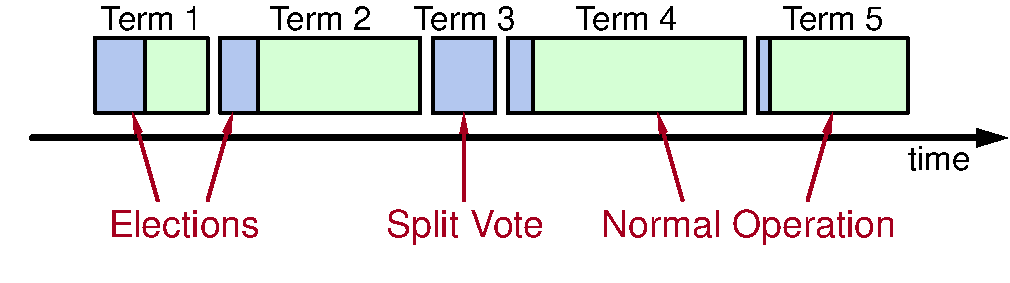
\includegraphics[width=0.80\columnwidth]{raft/terms}
	\caption{Un term è un priodo di tempo che parte con l'elezione di un nuovo leader e termina con la fine del suo "regno". 
		Un term attraversa normalmente due fasi: durante la prima, evidenziata in blu, i server eleggono il proprio leader; durante la seconda, evidenziata in verde, si svolgono le normali operazioni coordinate dal leader in carica.
		Non è possibile che due candidati ottengano la maggioranza all'interno dello stesso term, tuttavia è possibile che l'elezione si concluda in parità, come nel Term 3 in figura. In questo caso il term si conclude e ne inizia uno nuovo in cui si avvia una nuova elezione.}
	\label{fig:figure3}
\end{figure}


\begin{figure}[H]
	\centering
	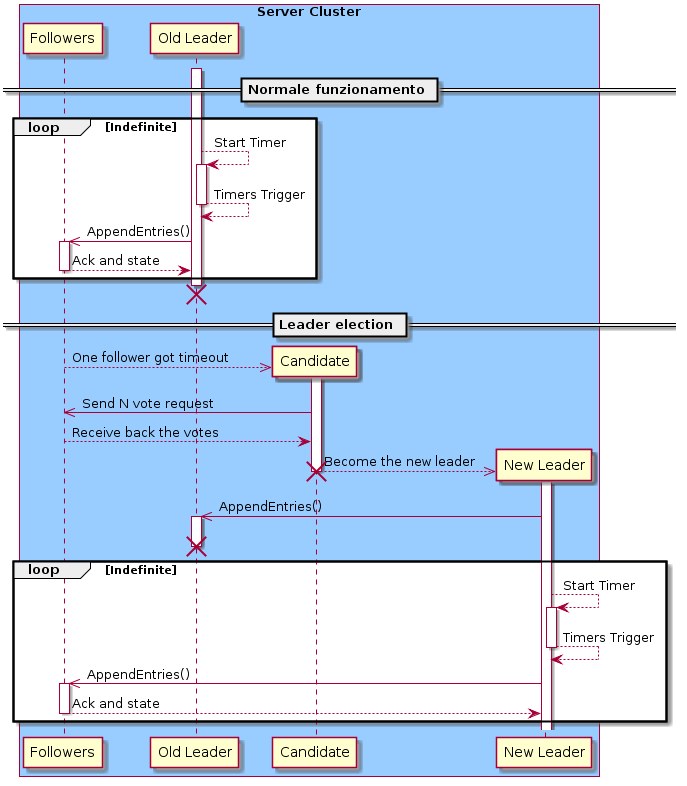
\includegraphics[width=0.80\columnwidth]{seqDiagrams/LeaderElection}
	\caption{Uno scenario semplificato in cui viene mostrata una \textit{Leader Election}. Il vecchio \textbf{Leader} inizialmente svolge correttamente le sue mansioni, divulgando periodicamente i propri \textit{heartbeats}; successivamente non riesce più a svolgere le sue attività. Prima o poi, non ricevendo più notizie dal leader, uno dei \textbf{Follower} vedrà scadere il proprio timer. Diventato \textbf{Candidate}, esso procederà a inviare le \textit{Vote request} a tutti i follower del cluster. Ricevuta la maggioranza dei voti verrà eletto \textbf{Leader} e ripristinerà il normale funzionamento del cluster. Il vecchio \textbf{Leader} quando tornerà on-line riceverà un AppendEntry e tornerà allo stato di \textbf{Follower}.}
	\label{fig:figure4}
\end{figure}


